% Author: Magdalen Berns

\chapter{The Physiology of The Eye}

\label{anatomy}

\section{A Normal Healthy Eye}
\label{anatomy}

The cornea is a transparent layer around 0.6mm thick, which curves over
the iris of the eye over its anterior chamber.
\cite{yaylali1997corneal,thoft1983x,patel1994refractive}
With a mean refractive index of around 1.4 (about the same as water),
the cornea allows plenty of light to pass through, but refracts as a
convergent lens due to its convex, shape. \Eref{eq:refractive} shows
Snell's Law of refraction for a light wave passing through two different
isotropic materials which have refractive indices $n_1$
and $n_2$, respectively.

\begin{figure}[htbp]
  \centering
    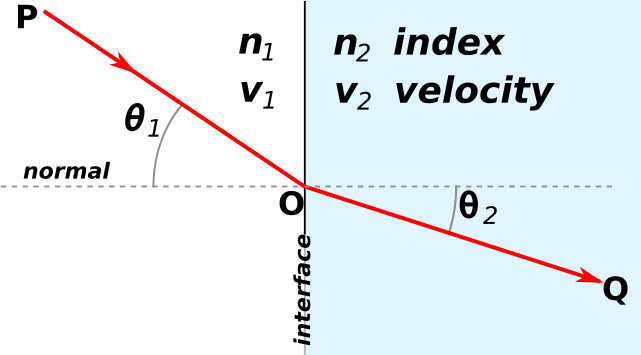
\includegraphics{figures/snells}
  \caption{Snell's law for diffraction at an interface where $n_1$ \textless $n_2$}
  \label{fig:snell}
\end{figure}

The angle $\theta_1$ is normal to the boundary between $n_1$ and $n_2$
and the angle $\theta_2$ is normal to the boundary between $n_2$ and $n_1$
as shown in \fref{fig:snell}

\begin{equation}
n_1\sin\theta_1=n_2\sin\theta_2
\label{eq:refractive}
\end{equation}

The radius of the human cornea tends to decrease with age and the cornea
itself, takes on a more spherical shape.\cite{guirao2000optical} Its
outermost surface is made of epithelial cells which are continuously lost
and replaced.\cite{jester1999cellular,hassell2010molecular} The reproduction
of cells is facilitated in part by tear ducts, which  serve to moisten the
eyes and remove harmful bacteria.\cite{holly1977tear}

There is a small circular opening in the iris, (the coloured section of
the eye) the pupil, has an aperture which dilates to allow an appropriate
amount of refracted light to pass through the lens. Light is refracted
once again through the lens converges towards a focal point on the back
of the eye. The lens makers expression in \eref{eq:lens_makers} is an
expression described by the diagram in \fref{fig:convergent_lens} which
shows light passing through a convex lens for calculating the focal point,
$f$ of distances $S_1$ and $S_2$ either side of a given convex lens.\cite{greivenkamp2004field}

\begin{equation}
\frac{1}{S_1} + \frac{1}{S_2} = \frac{1}{f}
\label{eq:lens_makers}
\end{equation}

\begin{figure}[htbp]
  \centering
    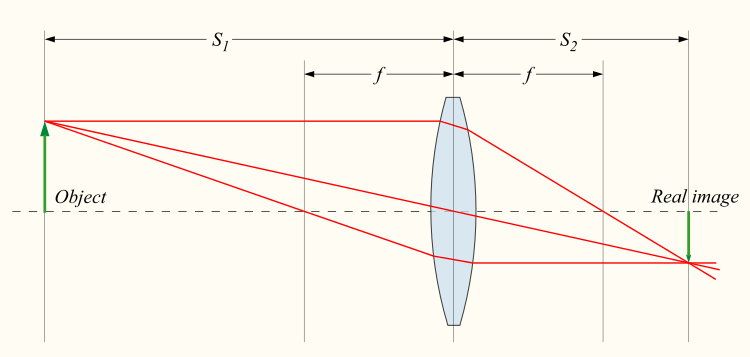
\includegraphics{figures/convergent_lens2}
  \caption{light passing through a convex lens for calculating the focal
  point, $f$ of distances $S_1$ and $S_2$ either side of a given convex lens.}
  \label{fig:convergent_lens}
\end{figure}

A ciliary body of tissue made up of fiber and muscle which accommodates the
lens and secretes a fluid, known as Aqueous Humour into a canal that flows
around the circumference of the eye called the Scleral Venous Sinus.
\cite{bill1970effects,dvorak1934schlemm}

When it becomes necessary to focus on objects at short distances, the
ciliary body muscles contract and suspensory ligaments attached to the
posterior chamber and the posterior lens to become taut, causing the
lens to become somewhat thicker in response to applied contractile
forces. When objects are far away the light is more parallel to the
lens' principle axis, less refraction is necessary, so the muscles
relax and suspensory ligaments attached to the posterior chamber and
the posterior lens so that it is no longer being accommodated so it
can take on a more rounded shape.

After photons of light leave the lens they pass through the vitreous
chamber, a clear substance, before they land onto the retina, which
is also transparent. A diagram which identifies the optic axis and
visual axis is shown in \fref{fig:optic_axis}.

The fovea

\begin{figure}[htbp]
  \centering
    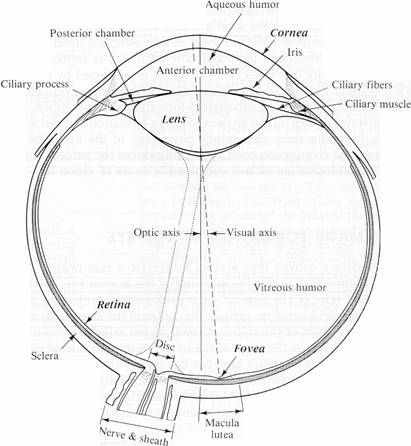
\includegraphics{figures/eye_diagram}
  \caption{A diagram of the eye which includes a visualisation of the visual
   and optic axis, the cornea, the retina and the fovea}
  \label{fig:optic_axis}
\end{figure}

The retina covers the entire receptive field of vision. It is supported by
the coroid, a vascular bed of tissues which supply the retina with blood and
removes toxins.\cite{} The retina is also supported by pigment cells.\cite{}

Just behind the retina are cones and rods which have photoreceptors so
that light can be converted into electrical signals and sent to the brain.
These signals can be transmitted to the brain via bunches of ganglion nerves.
Whilst cones are not particularly sensitive to light, they do aid to visual
acuity by granting us colour vision.\cite{}

A healthy and normal eye will pick up the full spectrum of colours.
\fref{fig:wavelengths} shows normalised absorbency against wavelength
for red, green and blue cones and rods (which cannot differentiate between
colours), in an average, human eye.

\begin{figure}[htbp]
  \centering
    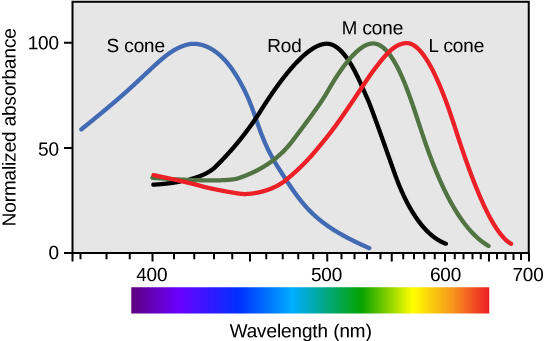
\includegraphics{figures/wavelengths}
  \caption{Normalised absorbency vs. wavelength, for an average eye.}
  \label{fig:wavelengths}
\end{figure}

\section{Birth, Development and Ageing}

As humans age, ciliary muscles weaken and this impairs the ciliary
muscles' ability to accommodate the lens and the result of this is
difficulty focusing at near distances.\cite{fisher1985ciliary}

Macular degeneration of pigment cells  is
also a common problem for the aged.

Preliminary studies show that the thickness of the coroid decreases
with age, but little is understood about how this may affect vision.
\cite{margolis2009pilot}

If all the eye cones are not working then this causes blindness
to occur.\cite{}